\documentclass[12pt,a4paper]{article}

\usepackage[utf8]{inputenc}
\usepackage[T1]{fontenc}
\usepackage[french]{babel}
\usepackage{geometry}
\usepackage{graphicx}
\usepackage{booktabs}
\usepackage{amsmath}
\usepackage{amssymb}
\usepackage{hyperref}
\usepackage{xcolor}
\usepackage{float}
\usepackage{caption}
\usepackage{subcaption}
\usepackage{array}
\usepackage{multirow}
\usepackage{parskip}

\geometry{margin=2.5cm}

\hypersetup{
    colorlinks=true,
    linkcolor=blue,
    urlcolor=blue,
}

\title{\textbf{REINFORCE et ses variantes}\\
\large Section du rapport — Apprentissage par renforcement}
\author{Moncef Benyamina}
\date{Avril 2026}

\begin{document}

\maketitle
\tableofcontents
\newpage

% ─────────────────────────────────────────────────────────────────────────────
\section{Description des algorithmes}
% ─────────────────────────────────────────────────────────────────────────────

\subsection{REINFORCE (Gradient de politique Monte-Carlo)}

REINFORCE (Williams, 1992) est l'algorithme fondateur des méthodes de gradient de politique (\textit{policy gradient}). Contrairement aux méthodes basées sur la valeur (Q-learning, DQN...), REINFORCE optimise directement la politique $\pi_\theta(a|s)$ paramétrée par un réseau de neurones, sans passer par une fonction de valeur intermédiaire.

L'idée centrale repose sur le théorème du gradient de politique (\textit{policy gradient theorem}) :

\[
\nabla_\theta J(\theta) = \mathbb{E}_{\tau \sim \pi_\theta}\left[\sum_{t=0}^{T} \nabla_\theta \log \pi_\theta(a_t|s_t) \cdot G_t\right]
\]

où $G_t = \sum_{k=t}^{T} \gamma^{k-t} r_k$ est le \textbf{retour cumulé actualisé} à partir du pas $t$, et $\gamma \in [0,1]$ est le facteur d'actualisation.

L'algorithme procède en épisodes complets (Monte-Carlo) :
\begin{enumerate}
    \item Jouer un épisode entier en suivant $\pi_\theta$ et enregistrer $(s_t, a_t, r_t)_{t=0}^T$
    \item Calculer les retours $G_t$ pour chaque pas de temps
    \item Mettre à jour les paramètres par descente de gradient stochastique :
    \[
    \theta \leftarrow \theta + \alpha \sum_{t=0}^{T} \nabla_\theta \log \pi_\theta(a_t|s_t) \cdot G_t
    \]
\end{enumerate}

En pratique, la fonction de perte minimisée est :
\[
\mathcal{L}(\theta) = -\sum_{t=0}^{T} \log \pi_\theta(a_t|s_t) \cdot G_t
\]

La politique est représentée par un réseau de neurones entièrement connecté (\textit{PolicyNetwork}) avec \textbf{masquage des actions illégales} (valeur $-\infty$ avant softmax).

\textbf{Avantage} : simplicité, convergence vers un optimum local garantie sous conditions de régularité.\\
\textbf{Inconvénient principal} : forte variance des gradients, ralentissant la convergence.

\subsection{REINFORCE avec Baseline Moyenne (Mean Baseline)}

Pour réduire la variance sans introduire de biais, on soustrait une \textbf{baseline} $b$ au retour :

\[
\mathcal{L}(\theta) = -\sum_{t=0}^{T} \log \pi_\theta(a_t|s_t) \cdot (G_t - b)
\]

La baseline choisie est la \textbf{moyenne des retours de l'épisode} :

\[
b = \frac{1}{T+1} \sum_{t=0}^{T} G_t
\]

Cette baseline préserve l'absence de biais (le gradient reste en espérance identique), tout en centrant les avantages autour de zéro. Les actions dont le retour est supérieur à la moyenne sont renforcées, les autres sont affaiblies.

\subsection{REINFORCE avec Réseau Critique (Actor-Critic)}

Cette variante remplace la baseline constante par une \textbf{estimation apprise} de la fonction de valeur $V^\pi(s)$ via un second réseau (\textit{ValueNetwork}). L'avantage estimé est :

\[
A_t = G_t - V(s_t; w)
\]

La perte totale combine la perte de l'acteur et celle du critique :

\[
\mathcal{L} = \underbrace{-\sum_t \log \pi_\theta(a_t|s_t) \cdot A_t}_{\text{perte acteur}} + \; \alpha_v \underbrace{\sum_t \left(G_t - V(s_t; w)\right)^2}_{\text{perte critique (MSE)}}
\]

Un seul optimiseur Adam est utilisé pour les deux réseaux. Le gradient de la perte acteur est \textbf{stoppé} sur les valeurs du critique (\texttt{.detach()}) pour éviter toute interférence.

% ─────────────────────────────────────────────────────────────────────────────
\section{Architecture et hyperparamètres}
% ─────────────────────────────────────────────────────────────────────────────

\subsection{Architecture du réseau de neurones}

\begin{table}[H]
\centering
\caption{Architecture de la \textit{PolicyNetwork} (partagée par les 3 variantes)}
\begin{tabular}{ll}
\toprule
\textbf{Couche} & \textbf{Détail} \\
\midrule
Entrée & $\dim(s)$ neurones (taille de l'espace d'état) \\
Couche cachée 1 & 128 neurones, activation ReLU \\
Couche cachée 2 & 128 neurones, activation ReLU \\
Sortie & $|\mathcal{A}|$ neurones (logits), masquage des actions illégales \\
\bottomrule
\end{tabular}
\end{table}

La \textit{ValueNetwork} (REINFORCE Critic uniquement) a la même architecture avec une sortie scalaire (sans activation).

\subsection{Hyperparamètres}

\begin{table}[H]
\centering
\caption{Hyperparamètres communs aux 3 variantes REINFORCE}
\begin{tabular}{lll}
\toprule
\textbf{Hyperparamètre} & \textbf{Valeur} & \textbf{Description} \\
\midrule
\texttt{gamma} & 0.99 & Facteur d'actualisation \\
\texttt{lr} & 0.001 & Taux d'apprentissage (Adam) \\
\texttt{hidden\_sizes} & [128, 128] & Taille des couches cachées \\
\texttt{value\_coef} & 0.5 & Pondération perte critique (Critic uniquement) \\
\texttt{max\_norm} & 1.0 & Seuil de gradient clipping \\
Optimiseur & Adam & Pour acteur et critique \\
Seed & 42 & Reproductibilité \\
\bottomrule
\end{tabular}
\end{table}

\begin{table}[H]
\centering
\caption{Budget d'entraînement par environnement}
\begin{tabular}{lll}
\toprule
\textbf{Environnement} & \textbf{Épisodes} & \textbf{max\_steps/épisode} \\
\midrule
LineWorld  & 100\,000 & 50  \\
GridWorld  & 10\,000  & 100 \\
TicTacToe  & 100\,000 & 50  \\
Bobail     & 100\,000 & 200 \\
\bottomrule
\end{tabular}
\end{table}

% ─────────────────────────────────────────────────────────────────────────────
\section{Résultats}
% ─────────────────────────────────────────────────────────────────────────────

Les métriques sont calculées lors d'évaluations périodiques (tous les 500 épisodes, sur 500 épisodes de test en mode greedy).

\subsection{LineWorld}

LineWorld est un environnement déterministe unidimensionnel. L'agent doit atteindre l'extrémité droite en exactement 2 pas optimaux.

\begin{table}[H]
\centering
\caption{Résultats sur LineWorld (100\,000 épisodes)}
\begin{tabular}{llcc}
\toprule
\textbf{Agent} & \textbf{Épisodes} & \textbf{Score moyen} & \textbf{Longueur moy.} \\
\midrule
REINFORCE        & 1\,000   & \textbf{1.000} & 2.0 \\
REINFORCE        & 10\,000  & \textbf{1.000} & 2.0 \\
REINFORCE        & 100\,000 & \textbf{1.000} & 2.0 \\
\midrule
REINFORCE MB     & 1\,000   & \textbf{1.000} & 2.0 \\
REINFORCE MB     & 10\,000  & \textbf{1.000} & 2.0 \\
REINFORCE MB     & 100\,000 & \textbf{1.000} & 2.0 \\
\midrule
REINFORCE Critic & 1\,000   & \textbf{1.000} & 2.0 \\
REINFORCE Critic & 10\,000  & \textbf{1.000} & 2.0 \\
REINFORCE Critic & 100\,000 & \textbf{1.000} & 2.0 \\
\bottomrule
\end{tabular}
\end{table}

\subsection{GridWorld}

GridWorld est un environnement en grille 2D avec obstacles. La longueur optimale est de 8 pas.

\begin{figure}[H]
\centering
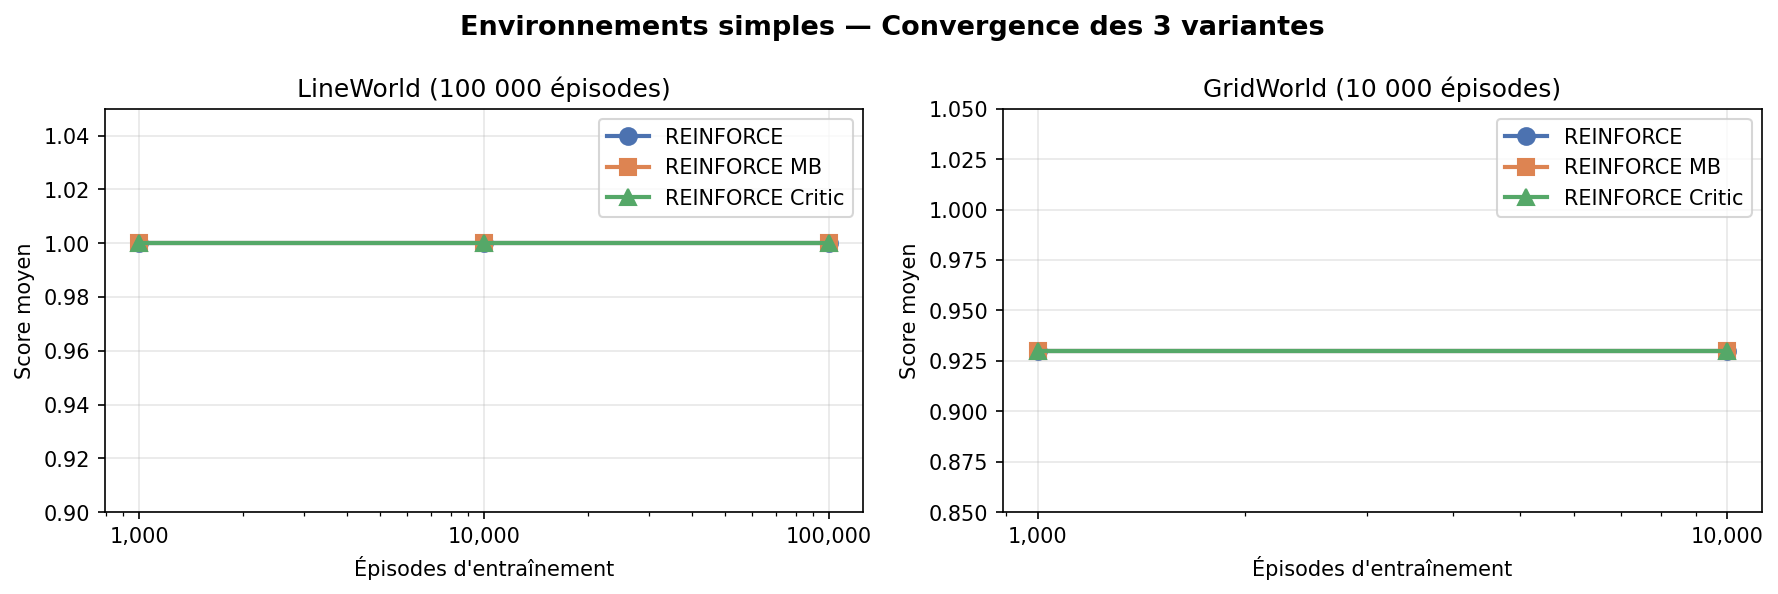
\includegraphics[width=\textwidth]{figures_reinforce/simple_envs.png}
\caption{Convergence des 3 variantes REINFORCE sur LineWorld et GridWorld}
\end{figure}

\begin{table}[H]
\centering
\caption{Résultats sur GridWorld (10\,000 épisodes)}
\begin{tabular}{llcc}
\toprule
\textbf{Agent} & \textbf{Épisodes} & \textbf{Score moyen} & \textbf{Longueur moy.} \\
\midrule
REINFORCE        & 1\,000  & \textbf{0.930} & 8.0 \\
REINFORCE        & 10\,000 & \textbf{0.930} & 8.0 \\
\midrule
REINFORCE MB     & 1\,000  & \textbf{0.930} & 8.0 \\
REINFORCE MB     & 10\,000 & \textbf{0.930} & 8.0 \\
\midrule
REINFORCE Critic & 1\,000  & \textbf{0.930} & 8.0 \\
REINFORCE Critic & 10\,000 & \textbf{0.930} & 8.0 \\
\bottomrule
\end{tabular}
\end{table}

Les trois variantes convergent vers un score de \textbf{0.930} dès les 1\,000 premiers épisodes avec une longueur stable à 8.0 (chemin optimal). La faible complexité de ces deux environnements ne permet pas de distinguer les variantes entre elles.

\subsection{TicTacToe}

TicTacToe est un jeu à deux joueurs à somme nulle. L'agent (Joueur X) affronte un adversaire aléatoire.

\begin{figure}[H]
\centering
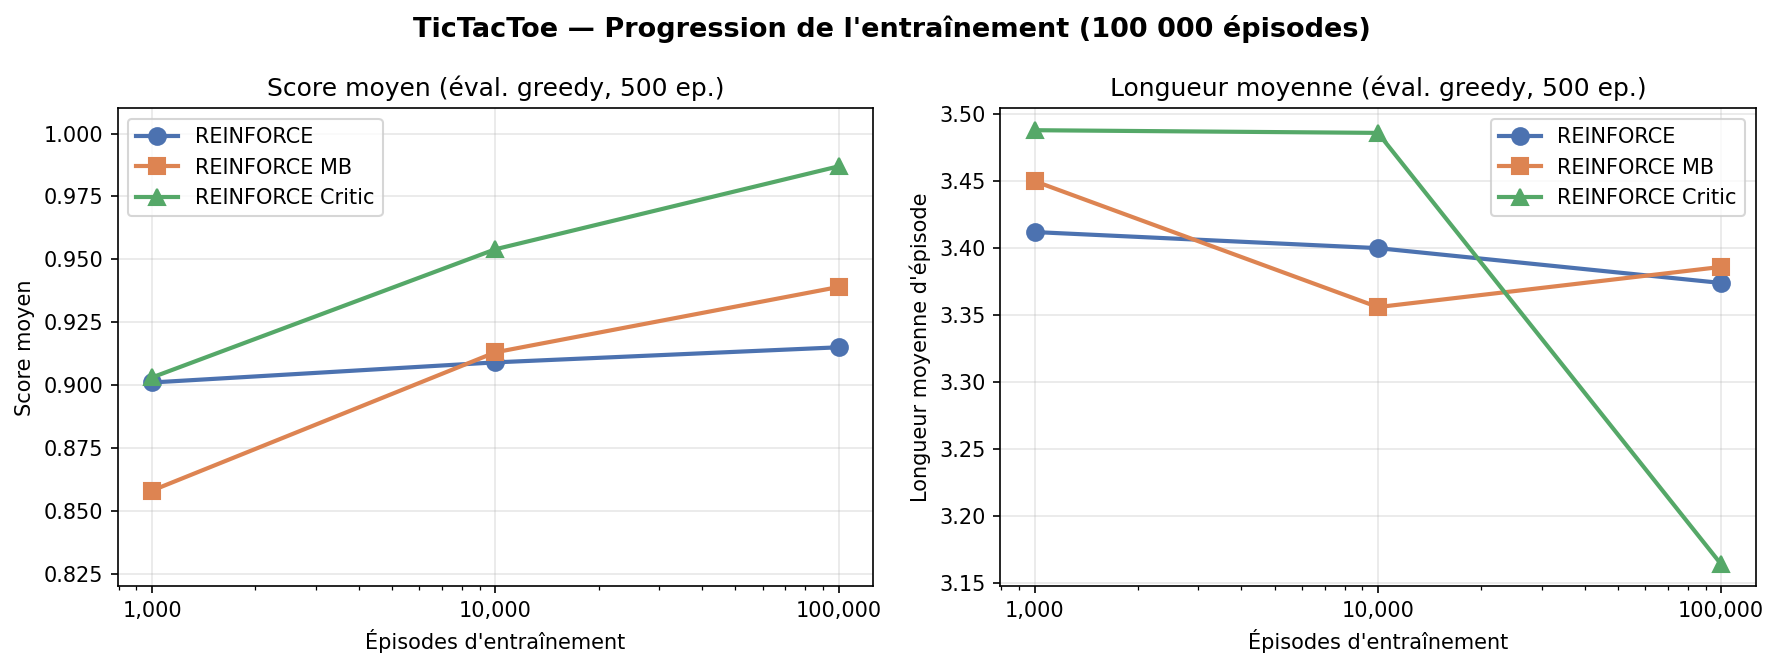
\includegraphics[width=\textwidth]{figures_reinforce/tictactoe_progression.png}
\caption{Progression du score moyen et de la longueur d'épisode sur TicTacToe}
\end{figure}

\begin{table}[H]
\centering
\caption{Résultats sur TicTacToe (100\,000 épisodes)}
\begin{tabular}{llcc}
\toprule
\textbf{Agent} & \textbf{Épisodes} & \textbf{Score moyen} & \textbf{Longueur moy.} \\
\midrule
REINFORCE        & 1\,000   & 0.901 & 3.412 \\
REINFORCE        & 10\,000  & 0.909 & 3.400 \\
REINFORCE        & 100\,000 & 0.915 & 3.374 \\
\midrule
REINFORCE MB     & 1\,000   & 0.858 & 3.450 \\
REINFORCE MB     & 10\,000  & 0.913 & 3.356 \\
REINFORCE MB     & 100\,000 & 0.939 & 3.386 \\
\midrule
REINFORCE Critic & 1\,000   & 0.903 & 3.488 \\
REINFORCE Critic & 10\,000  & 0.954 & 3.486 \\
REINFORCE Critic & 100\,000 & \textbf{0.987} & \textbf{3.164} \\
\bottomrule
\end{tabular}
\end{table}

TicTacToe est le premier environnement qui discrimine clairement les trois variantes :

\begin{itemize}
    \item \textbf{REINFORCE} progresse lentement (+1.4 pts en 99\,000 épisodes). La forte variance des gradients Monte-Carlo freine l'apprentissage.
    \item \textbf{REINFORCE Mean Baseline} montre une progression plus marquée grâce au centrage des avantages, atteignant 0.939 (+2.4 pts vs REINFORCE à budget égal).
    \item \textbf{REINFORCE Critic} obtient les meilleures performances avec \textbf{0.987}, une politique quasi-parfaite contre un adversaire aléatoire. La longueur de 3.164 (contre $\sim$3.4 pour les autres) indique une stratégie plus agressive.
\end{itemize}

\subsection{Bobail}

Bobail est un jeu de plateau 5$\times$5 à deux joueurs. L'agent (Joueur 0) affronte un adversaire aléatoire.

\begin{figure}[H]
\centering
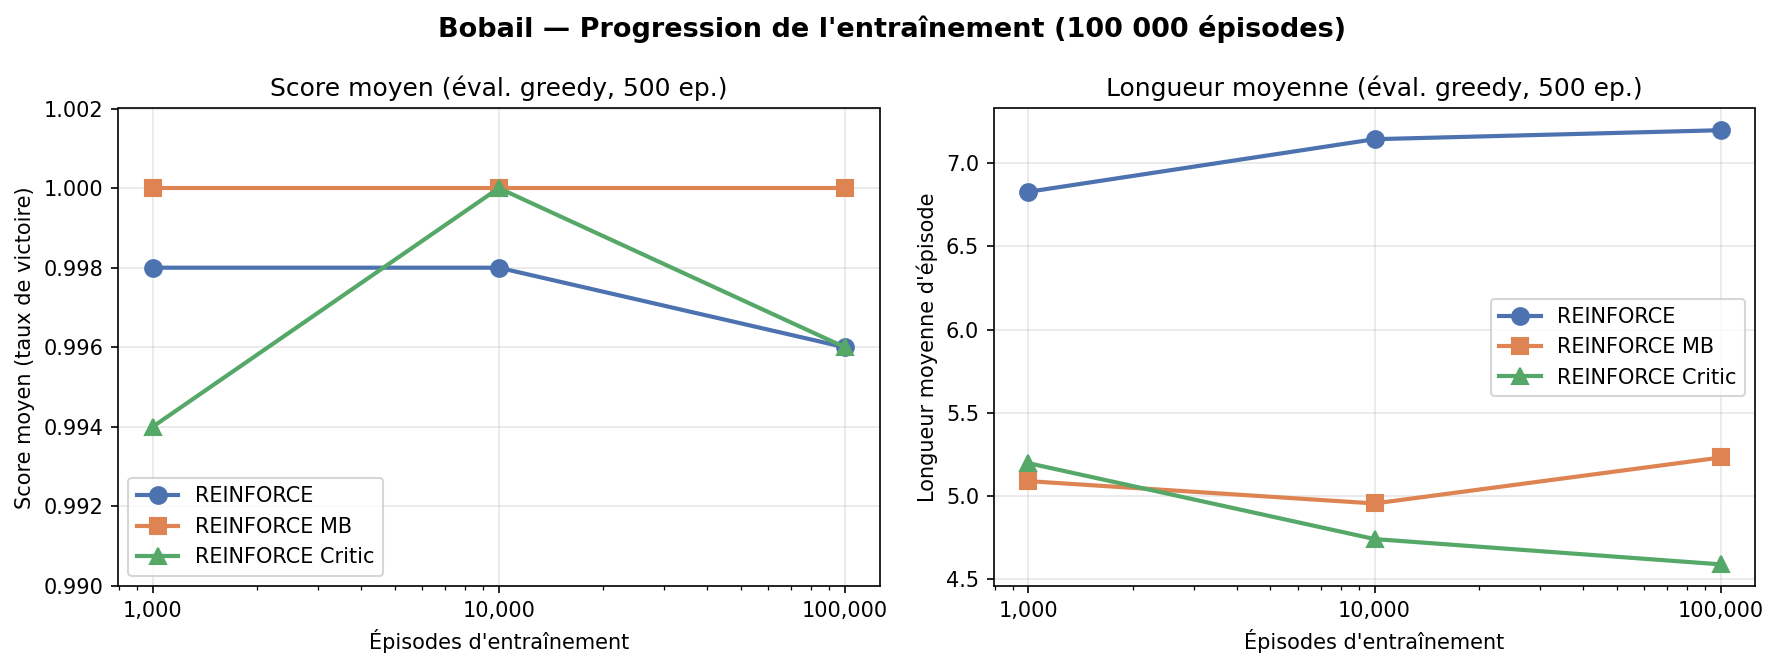
\includegraphics[width=\textwidth]{figures_reinforce/bobail_progression.png}
\caption{Progression du score moyen et de la longueur d'épisode sur Bobail}
\end{figure}

\begin{table}[H]
\centering
\caption{Résultats sur Bobail (100\,000 épisodes). * ré-entraîné sur l'environnement corrigé.}
\begin{tabular}{llcc}
\toprule
\textbf{Agent} & \textbf{Épisodes} & \textbf{Score moyen} & \textbf{Longueur moy.} \\
\midrule
REINFORCE        & 1\,000   & 0.998 & 6.828 \\
REINFORCE        & 10\,000  & 0.998 & 7.144 \\
REINFORCE        & 100\,000 & 0.996 & 7.198 \\
\midrule
REINFORCE MB     & 1\,000   & \textbf{1.000} & 5.090 \\
REINFORCE MB     & 10\,000  & \textbf{1.000} & 4.956 \\
REINFORCE MB     & 100\,000 & \textbf{1.000} & 5.232 \\
\midrule
REINFORCE Critic* & 1\,000   & 0.994 & 5.198 \\
REINFORCE Critic* & 10\,000  & \textbf{1.000} & 4.742 \\
REINFORCE Critic* & 100\,000 & 0.996 & \textbf{4.590} \\
\bottomrule
\end{tabular}
\end{table}

\textit{* REINFORCE Critic a été ré-entraîné sur la version corrigée de l'environnement Bobail (state\_size=78, avec le bit \texttt{first\_turn}) suite à la correction des règles du premier tour.}

\vspace{0.5em}

REINFORCE MB atteint un score parfait de \textbf{1.000} dès 1\,000 épisodes et le maintient. REINFORCE sans baseline n'atteint jamais 1.000, confirmant l'impact négatif de la variance sur les environnements complexes. REINFORCE Critic se distingue par la \textbf{longueur la plus courte} (4.590 à 100\,000 épisodes), signe d'une stratégie plus directe et agressive.

% ─────────────────────────────────────────────────────────────────────────────
\section{Synthèse comparative}
% ─────────────────────────────────────────────────────────────────────────────

\begin{figure}[H]
\centering
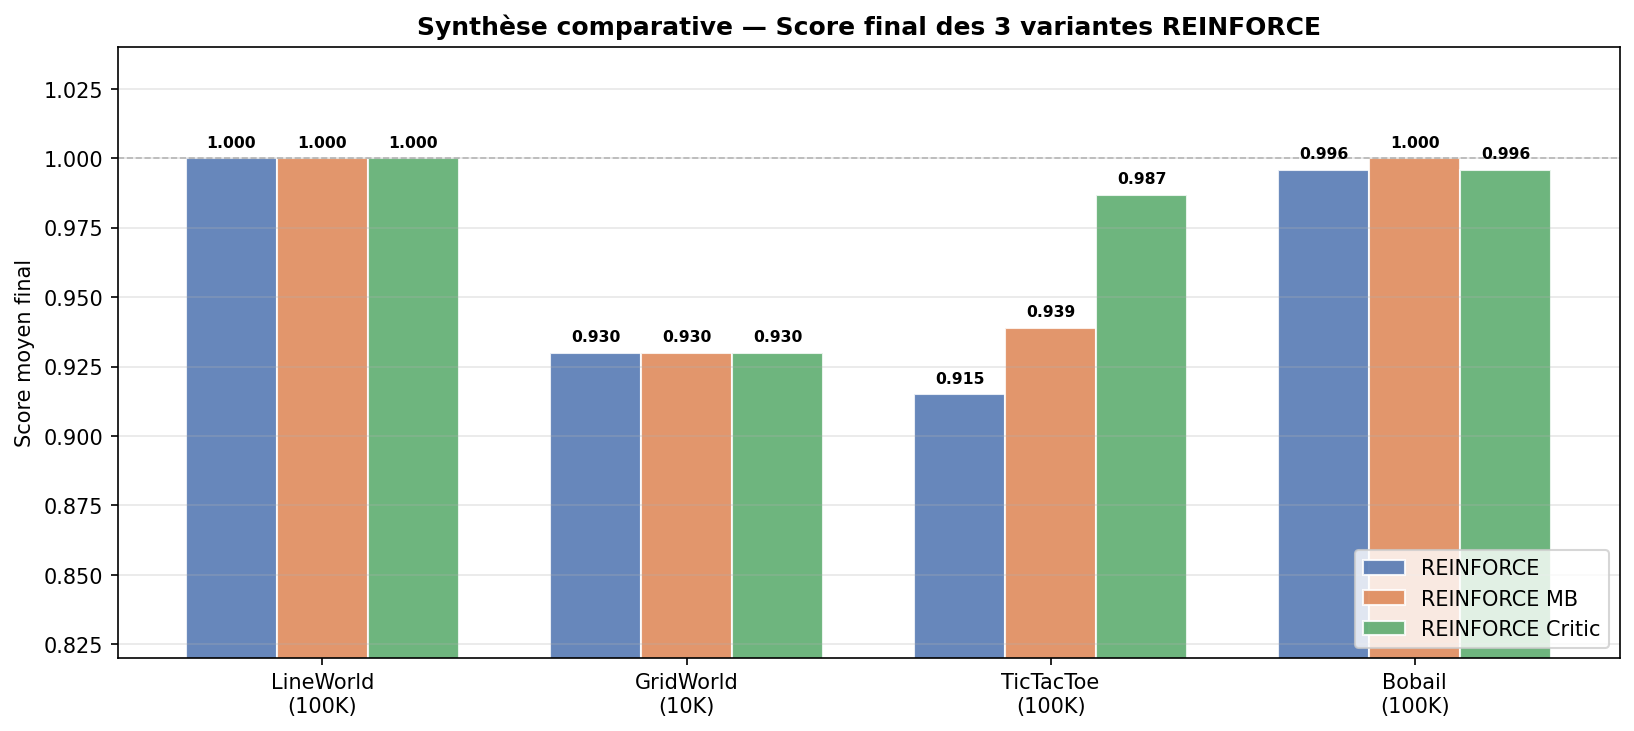
\includegraphics[width=\textwidth]{figures_reinforce/summary_bar_chart.png}
\caption{Comparaison des scores finaux des 3 variantes REINFORCE sur les 4 environnements}
\end{figure}

\begin{table}[H]
\centering
\caption{Scores finaux (checkpoint 100\,000 épisodes, sauf GridWorld : 10\,000)}
\begin{tabular}{lccc}
\toprule
\textbf{Environnement} & \textbf{REINFORCE} & \textbf{REINFORCE MB} & \textbf{REINFORCE Critic} \\
\midrule
LineWorld  & 1.000 & 1.000 & 1.000 \\
GridWorld  & 0.930 & 0.930 & 0.930 \\
TicTacToe  & 0.915 & 0.939 & \textbf{0.987} \\
Bobail     & 0.996 & \textbf{1.000} & 0.996 \\
\bottomrule
\end{tabular}
\end{table}

\textbf{Conclusions principales :}

\begin{enumerate}
    \item Sur les environnements simples (LineWorld, GridWorld), les trois variantes convergent vers des performances identiques. La variance n'est pas un facteur limitant.
    \item Sur TicTacToe, la réduction de variance fait une différence significative : REINFORCE Critic (+7.2 pts) $>$ REINFORCE MB (+2.4 pts) $>$ REINFORCE.
    \item Sur Bobail, REINFORCE MB et REINFORCE Critic atteignent des performances quasi-parfaites. Le Critic se distingue par une stratégie plus rapide (longueur $\sim$4.59 contre $\sim$5.2).
    \item REINFORCE sans baseline est systématiquement le moins performant sur les environnements complexes, confirmant empiriquement l'impact de la variance des gradients Monte-Carlo.
    \item Les temps de décision restent inférieurs à 1.2 ms pour les trois variantes, ce qui les rend utilisables en temps réel.
\end{enumerate}

\end{document}
